\chapter{Design Motivation}
\label{ch:fddp-design}

%%%%%%%%%%%%%%%%%%%%%%%%%%%%%%%%%%%%%%%%%%%%%%%%%%%%%%%%%%%%%%%%%%%%
\section{Introduction to Dual-Phase Far Detector in DUNE}
\label{sec:fddp-design-highlight}

Similarly as for the Single-Phase design the DUNE Dual-Phase Far Detector is aiming at opening new windows of opportunity in the study
of neutrinos.  DUNE's rich physics program, with discovery potential for CP-Violation in the neutrino sector, and capability to make
significant observations of nucleon decay and astrophysical events, is enabled by the exquisite resolution of the LArTPC detector technique which is further augmented in the Dual-Phase design. The Dual-Phase design allows for improving the signal to noise ratio in the charge readout and lowering thresholds for the smallest observable signals while achieving at the same time a finer readout granularity.  The Dual-Phase technology aims at building larger drift volumes, reducing so the presence of dead materials in the liquid argon target. The basic physics requirements are identical for Single-Phase and Dual-Phase design with teh Dual-Phase design offering augmented performance under some aspects.

%%%%%%%%%%%%%%%%%%%%%%%%%%%%%%%%%%%%%%%%%%%%%%%%%%%%%%%%%%%%%%%%%%%%

\section{Dual-Phase LArTPC Operational Principle}
\label{sec:fddp-operational-principle}

The basic operational principle is very similar as for the Single-phase design. The precision tracking and calorimetry offered by the Dual-Phase LArTPC
technology provides excellent ability to identify interactions of interest while mitigating sources of background.  Charged particles traversing the active volume of the LArTPC ionize the medium, while also producing scintillation light.  The ionization drifts along an electric field that is present throughout the volume, towards a segmented anode.

The key concept of the Dual-Phase design relies on the possibility of amplifying the ionization signal in avalanche processes. In the Single-Phase design charges are drifted horizontally to the anode which is constituted by a set of induction and collection wire layers immersed in the liquid. In the Dual-Phase design electrons are drifted vertically towards an extraction grid just below the liquid-vapor interface. After reaching the grid, the electrons are extracted from the liquid to the gas phase thanks to an electric field stronger than the drift field. Once in the gas electrons can be amplified in avalanches occurring in high field regions present withing micro-pattern gas detectors, the Large Electron Multipliers (LEM). The amplified electrons are then eventually collected on a finely segmented anode with two perpendicular collection views. 

The DUNE Dual-Phase LArTPC detector design foresees a single, fully homogeneous, liquid argon volume with a long drift. This volume is surrounded at the sides and at the bottom by a field cage and a cathode, which define the drift field. At the top of the detector, the anode is constituted by a set of active detector elements Charge Readout Planes (CRP), located in the gas phase. The CRP integrate the LEM and anodes and support the extraction grid which is immersed in the liquid. They can be individually positioned at a few millimeters parallel to the interface between the liquid and the gas ensuring that the extraction grid is immersed.

The argon scintillation light, which at 128 nm wavelength is deep in the UV spectrum, can be recorded by an array of photomultipliers, located below the cathode. The photomultipliers are coated with a material that shifts the wavelength closer to the visible spectrum and subsequently record the time and
pulse characteristics of the incident light.

The performance of the  LArTPC hinges on several key factors.  First, the purity of the liquid argon must be extremely high in order for ionization to
be able to drift over several meters towards the anode planes.  The levels of electronegative contaminants (e.g. oxygen, water), must be reduced and
maintained to $\sim$ppt levels in order to achieve minimum charge attenuation over the longest drift lengths in the LArTPC.   Second, the electronic readout
of the LArTPC requires very low noise levels so that the signal of drifting ionization is clearly discernible over the baseline of the electronics.  The Dual-Phase design relies on the same purity requirements as for Single-Phase and on the use of low noise cryogenic electronics. However the impact of these aspects on the performance is mitigated by the possibility of amplifying the electrons signal in the gas phase. On the other hand the Dual-Phase design requires higher voltages to be applied to the cathode in order to define the drift field over longer paths.

\begin{dunefigure}[optional caption for LoF]{fig:figure-label-DPprinciple}{Principle of the Dual-Phase readout}
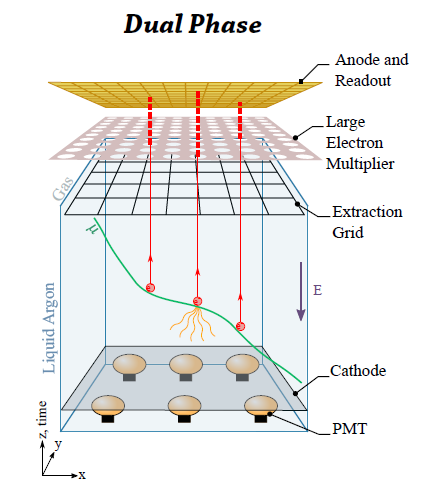
\includegraphics[width=0.6\textwidth]{dualphase-principle}
\end{dunefigure}

\section{Motivation of Dual-Phase LArTPC Design at DUNE}
\label{sec:fddp-design-motivation}

The innovative Dual-Phase design is similar in many ways to the Single-Phase design, but implements some unique features and offers several advantages over it, in particular the electron amplification in the gas phase enables a robust and tunable signal-to-noise ratio.  The features of the Dual-Phase design, e.g., high gain,  allow achieving very long drift paths, compensating for losses due to electronegative impurities, and large detector dimensions while minimizing the number of readout channels, thanks to the long projective geometry.  In addition a Dual-Phase DUNE far detector is built out of a smaller number of construction modules and readout channels than an equivalent Single-Phase Far Detector module. The detector design provides other practical advantages such as the full accessibility to all the front-end electronics which can be replaced at any time while the detector is operating without contaminating the liquid argon volume. All these aspects, providing an appealing and complementary approach to the Single-Phase design, as summarized below:

\begin{itemize}
\item  Higher, tunable, gain, leading to a larger signal-to-noise ratio (S/N);
\item  Lower detection threshold;
\item  Larger fiducial volume, enabling very long drift paths;
\item  Absence of dead material in the LAr drift volume;
\item  Finer readout pitch (3~mm), implemented in two identical collection views, $x$ and $y$;
\item  Fewer readout channels than an equivalent Single-Phase Far Detector (153,600 (DP) vs 384,000 (SP) for a reference design \ktadj{10} module); 
\item  Full accessibility and replaceability of the front-end electronics during the detector operation.
\end{itemize}

 The Dual-Phase design features maximize the capability of the experiment and are motivated to cope with the the unprecedented scale of the Far Detector modules and the deep underground location where construction will occur.

Among the features driven by the underground location of the experiment, all detector components are sized to fit within the constraints of the SURF shafts and access pathways. The CRP modules are essentially planar objects with a surface of $3 \times 3$ $m^2$. All the other detector modules (field cage and cathode modules) are as well designed in order to stay within this envelope. The relatively small number of detector elements makes easier the underground installation

A drift time of several milliseconds is typical for ionization to arrive at the anode wires after drifting several meters.  This lengthy duration of time, as well as aspects of the DUNE Physics program looking for rare and low-energy processes, makes the deep underground location essential for the DUNE-DP detector.  The overburden of $\sim$1 mile of earth will vastly reduce the rate of cosmic-rays reaching the active volume of the DUNE-DP detector, greatly enhancing the ability to search for rare and low-energy signatures without the influence of cosmic-induced backgrounds.  





